\documentclass{article}
\usepackage[utf8]{inputenc}
\usepackage{amsmath,amsthm,amssymb}
\usepackage{amsfonts}
\usepackage{arydshln}
\usepackage{cases}
\usepackage{enumitem}
\usepackage{float}
\usepackage{graphicx}
\usepackage{hyperref}
\usepackage{listings}
\usepackage{makecell}
\usepackage[margin=0.75in]{geometry}
\usepackage{multicol}
\usepackage{subcaption}
\usepackage{titlesec}
\usepackage{wrapfig}
\allowdisplaybreaks
\newtheorem{theorem}{Theorem}
\newtheorem{lemma}{Lemma}

\usepackage{fancyhdr}
\pagestyle{fancy}
\fancyhf{}
\fancyhead[L]{Bridgette Delight}
\fancyhead[C]{Math 465 - Homework 03}
\fancyhead[R]{pg. \thepage}
\renewcommand{\headrulewidth}{2pt}

\title{{\large Math 465}\\ Homework 03}
\author{Bridgette Delight}
\date{\today}

\begin{document}

\noindent Consider the function $F: \mathbb{R}^2 \to \mathbb{R}^2$ such that

\begin{numcases}{F(x,y)}=
    x^4-6x^2y^2+y^4-16 &\\ \label{case 1}
    4x^3y-4xy^3 & \label{case 2}
\end{numcases}

and the iterative scheme
\begin{equation}\label{eq:iterSch}
   \left( \begin{matrix}
x^{(k+1)}\\[1ex] 
y^{(k+1)}\\
\end{matrix}\right)
=    \left( \begin{matrix}
x^{(k)}\\[1ex]
y^{(k)}\\
\end{matrix}\right)
- \begin{bmatrix} J_F(x^{(k)},y^{(k)})
\end{bmatrix}^{-1}
\cdot F(x^{(k)},y^{(k)}), \quad k=0,1,2, \dots
\end{equation}
where $J_F$ is the Jacobian of $F$. Define the sets $S_1,S_2, \dots \subset \mathbb{R}^2$ such that 
$$S_i = \left\{(x^{(0)},y^{(0)})\in \mathbb{R}^2: \quad (x^{(k)},y^{(k)}) \to \xi_i \text{ as } k \to \infty \right\}, \quad i=1,2,3, \dots ,$$
where $\xi_1,\xi_2, \dots \in \mathbb{R}^2$ are roots of $F$.
\section{}
Determine a formula for $J_F(x,y)$.
\vspace{10mm}

$$\mathbf{J}_F(x,y) = \left[\frac{\partial F_i}{\partial x_j}(\xi)\right]_{i,j=1}^n$$
\[
\mathbf{J}_F(x,y) =
\begin{bmatrix}
  \frac{\partial F_1}{\partial x} & 
  \frac{\partial F_1}{\partial y}  \\[1ex] 
  \frac{\partial F_2}{\partial x} & 
  \frac{\partial F_2}{\partial y}  \\[1ex]
\end{bmatrix}
\]

\[
\mathbf{J}_F(x,y) =
\begin{bmatrix}
  4x^3-12xy^2 & -12x^2y+4y^3  \\[1ex] 
  12x^2y-4y^3 & 4x^3-12xy^2  \\[1ex]
\end{bmatrix}
\]


\section{}
Find the $3^{rd}$ iterate starting from $x^{(0)},y^{(0)}=(1,1)$.
\vspace{10mm}
\subsection*{First Iteration}
\[
\begin{pmatrix}
  x^{(1)}  \\[1ex] 
  y^{(1)}  \\[1ex]
\end{pmatrix}
=
\begin{pmatrix}
  x^{(0)}  \\[1ex] 
  y^{(0)}  \\[1ex]
\end{pmatrix}
-
\bigg[ J_F(x^{(0)}, y^{(0)})\bigg]^{-1}\cdot F(x^{0},y^{0})
\]

\[
\begin{pmatrix}
  x^{(1)}  \\[1ex] 
  y^{(1)}  \\[1ex]
\end{pmatrix}
=
\begin{pmatrix}
  1 \\[1ex] 
  1  \\[1ex]
\end{pmatrix}
-
\begin{bmatrix}
  -8 & -8 \\[1ex] 
  8 & -8
\end{bmatrix}^{-1}
\cdot 
\begin{pmatrix}
  -20 \\[1ex] 
  0 \\[1ex] 
\end{pmatrix}
\]

\[
\begin{pmatrix}
  x^{(1)}  \\[1ex] 
  y^{(1)}  \\[1ex]
\end{pmatrix}
=
\begin{pmatrix}
  -0.25 \\[1ex] 
  -0.25 \\[1ex] 
\end{pmatrix}
\]

\subsection*{Second Iteration}
\[
\begin{pmatrix}
  x^{(2)}  \\[1ex] 
  y^{(2)}  \\[1ex]
\end{pmatrix}
=
\begin{pmatrix}
  -0.25 \\[1ex] 
  -0.25  \\[1ex]
\end{pmatrix}
-
\begin{bmatrix}
  0.125 & 0.25 \\[1ex] 
  -0.125 & 0.125
\end{bmatrix}^{-1}
\cdot 
\begin{pmatrix}
  -16.015625 \\[1ex] 
  0 \\[1ex] 
\end{pmatrix}
\]
\[
\begin{pmatrix}
  x^{(2)}  \\[1ex] 
  y^{(2)}  \\[1ex]
\end{pmatrix}
=
\begin{pmatrix}
  63.8125 \\[1ex] 
  63.8125 \\[1ex] 
\end{pmatrix}
\]

\subsection*{Third Iteration}
\[
\begin{pmatrix}
  x^{(3)}  \\[1ex] 
  y^{(3)}  \\[1ex]
\end{pmatrix}
=
\begin{pmatrix}
  63.8125  \\[1ex] 
  63.8125  \\[1ex]
\end{pmatrix}
-
\begin{bmatrix}
  -2078773.947 & -2078773.947 \\[1ex] 
  2078773.947 & -2078773.947
\end{bmatrix}^{-1}
\cdot 
\begin{pmatrix}
  -66325897.25 \\[1ex] 
  0 \\[1ex] 
\end{pmatrix}
\]
\[
\begin{pmatrix}
  x^{(3)}  \\[1ex] 
  y^{(3)}  \\[1ex]
\end{pmatrix}
=
\begin{pmatrix}
  47.859 \\[1ex] 
  47.859 \\[1ex] 
\end{pmatrix}
\]


\section{}
Determine the roots of $F$ analytically, and compare with your answer to 2.
\vspace{10mm}

From Equation \ref{case 2}:
\begin{align*}
    0 &= 4xx^2y-4xyy^2\\
    0 &= 4xy(x^2-y^2)\\
    \text{So,}&\\
    &4xy = 0, \quad x^2-y^2=0\\
    &xy=0,\quad x^2=y^2\\
    \text{So,}
    x&=0\\
    y&=0 \\
\end{align*}
From Equation \ref{case 1}:
\begin{align*}
    0 &= x^4-6x^2y^2+y^4-16\\
    \text{Substitute } x=y&\\
    0 &=
\end{align*}



\section{}
How many iteration are sufficient to obtain an accuracy of $10^{-2}$?
\vspace{10mm}

\section{}
Prepare a figure displaying the sets $S_i$ graphically as subsets of $\mathbb{R}^2$ by considering the sets $A_i \subset \mathbb{R}^2$, for $i$, such that
$$A_i= \left\{ (x^{(0)},y^{(0)})\in \mathbb{R}^2: \quad \parallel (x^{(N)},y^{(N)})-\xi_i \parallel_{\infty} < \varepsilon\right\}, \quad i=1,2,3,\dots ,$$
where $\varepsilon = 10^{-5}$ and $N=10$. For each point $(x_i,y_j)=(-2 + i \Delta x, \quad -2+j \Delta y)$, where $\Delta x = 10^{-2}$, $\Delta y = 10^{-2}$, $i$, $j=0,1,2,\dots , 400$, such that $|det(J_F(x_i,x_j))|> 10^{-15}$, assign the color red if $(x_i,y_j)\in A_1$, green if $(x_i,y_j)\in A_2$, blue is $(x_i,y_j)\in A_3$, cyan if $(x_i,y_j)\in A_4$, and yellow otherwise. If $|det(J_F(x_i,x_j))| \le 10^{-15}$, assign the color black.
\vspace{10mm}

\begin{figure}[H]
    \centering
    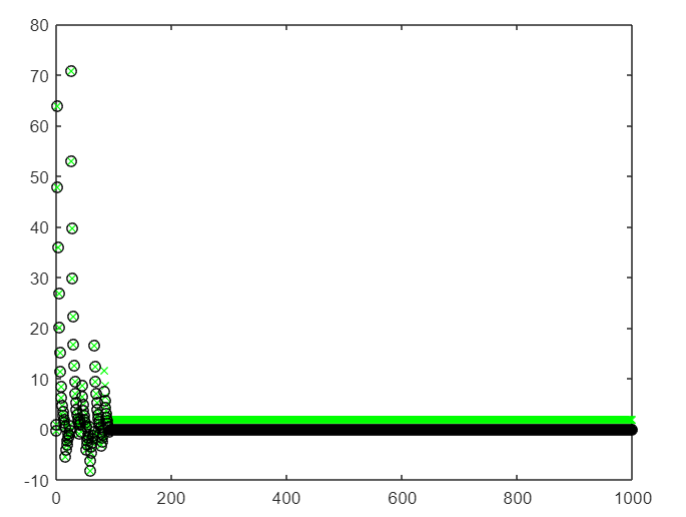
\includegraphics[width=.75\linewidth]{images/hw03q05.PNG}
    \caption{N=10}
    \label{fig:question5 n=10}
\end{figure}

\section{}
Prepare a figure displaying the sets $S_i$ when $N=20$. What happens then? Does the region colored yellow get smaller or larger? Why would you expect that?
\vspace{10mm}

\begin{figure}[H]
    \centering
    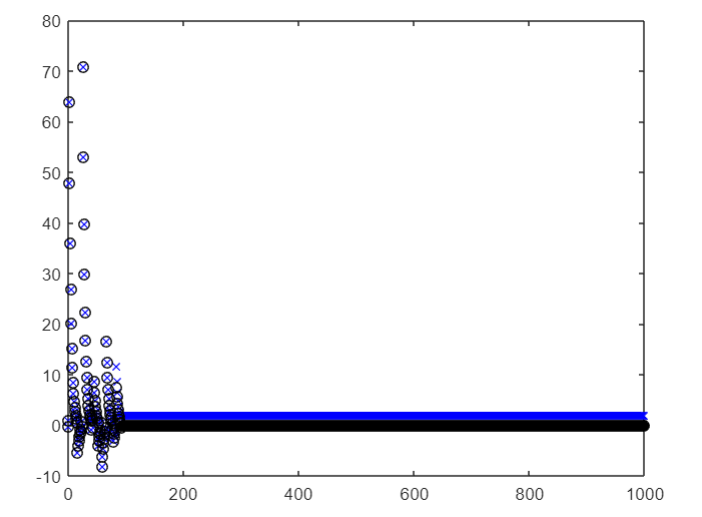
\includegraphics[width=.75\linewidth]{images/hw03q06.PNG}
    \caption{N=20}
    \label{fig:question6 n=20}
\end{figure}
\section{}
What do the figures that you generated in 5. and 6. indicate about the sensitivity of the iterative scheme (\ref{eq:iterSch}) to the choice of initial value $(x^{(0)},y^{(0)})$?
\vspace{10mm}






\end{document}